 % =================================== CHAPTER ===================================
\chapter{Дослідження систем захисту захищених месенджерів типу Telegram, Viber, WhatsApp, Signal}

Telegram, Signal, WhatsAPP, Viber є одними з найпопулярнiших месенджерiв у свiтi, якими користуються мiльйони людей. Як і кількість особистої інформації та кількість користувачів продовжує зростати щодня. Все бiльше людей проводять конфiденцiйнi розмови в месенджерах, сподіваючись, що ця iнформацiя залишиться приватною i недоступною для стороннiх осiб. Захищенi месенджери допомагають запобiгти кiберзлочинам, таким як шпигунство, крадiжка особистої iнформацiї, фiшинг або викрадення облiкових даних. Тож напевне треба знати які месенджери варто використовувати. У даному досліджені розглянемо популярні месенджери та їх механізми захисту інформації.

 % =================================== SECTION ===================================
\section{Telegram}

\begin{wrapfigure}{l}{0.25\textwidth}
    
\includegraphics[width=0.9\linewidth]{../IMAGES/telegram.png} 
    \label{fig:telegram}
\end{wrapfigure}

\textbf{Telegram} - хмарна, крос-платформена соціальна мережа, що має можливість швидким обміном повідомлень. Він дозволяє користувачам обмінюватися повідомленнями, ділитися файлами, проводити приватні групові, а також публічні трансляції. На даний час він став одним із найбільш завантажуваним додатком та має понад 500 мільйонів активних користувачів станом на 2021 рік.


Для того, щоб зрозуміти, чому Telegram не є E2E зашифрованим за замовчуванням треба згадати, що основою частиною функціоналу месенджера є:
\begin{itemize}
    \item Канали (one-to-many), які поширюють інформацію на загал. Канали у свою чергу можуть: 
        \begin{itemize}
            \item бути публічними чи приватними;
            \item мати необмежену кількість учасників;
            \item мати адміністраторів, що надсилають повідомлення всім, хто підписався.
        \end{itemize}
        Якщо узагальнити, то кожен може бачити повідомлення, а канал, по суті, діє як стрічка публікацій від адміністраторів. До прикладу, на каналі <<Мілітарний>> станом на кінець 2024 року є 63 тисячі підписників.
    \item Групові чати, що підтримують до 200 тисяч користувачів, які працють як у більшості інших месенджерів.
    \item Особисті \textit{хмарні} чати, у яких є компанія може показувати та синхронізувати повідомлення в програмах для комп’ютера та смартфона в реальному часі. Це також означає, що повідомлення, які надсилаються, зберігаються на її серверах – компанія каже, що повідомлення в хмарних чатах <<теоретично>> доступні.
    \item Особисті \textit{секретні} чати, що використовують E2E шифрування та не мають можливості синхронізації між пристроями, адже доступні лише на мобільних пристроях.
    \item Особисті голосові та відео дзвінки, що використовують протоколи які мають деяку схожість із секретними чатами. Вони не мають функції запису дзвінків, лише комунікація у реальному часі.
\end{itemize}


Спочатку поговорімо про \textbf{хмарні чати}. 

\textbf{MTProto v1} — це спеціальний мобільний протокол, розроблений командою Telegram \cite{telegram_mtproto1}, що був розкритикований численними експертами з криптографії. Організація вирішила не йти уже протоптаним шляхом та зробила свій стек протоколів для обміну повідомленнями за допомогою своєї комбінації шифрування. Додамо, що на даний час цей протокол не використовується, але був у викорстанні до 2021 року.

\begin{figure}[ht]
        \centering
        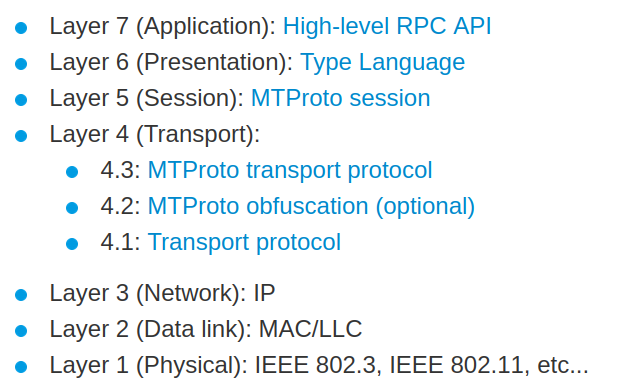
\includegraphics[scale=0.37]{../IMAGES/mproto_layers.png}
        \caption{Схема рівнів для MTProto v1.}
        \label{mproto_layers}
\end{figure}

\begin{remark}
    Як кажуть у суспільстві: <<Don't roll over your crypto>>, але Telegram зробив по іншому.
\end{remark}

\begin{figure}[ht]
        \centering
        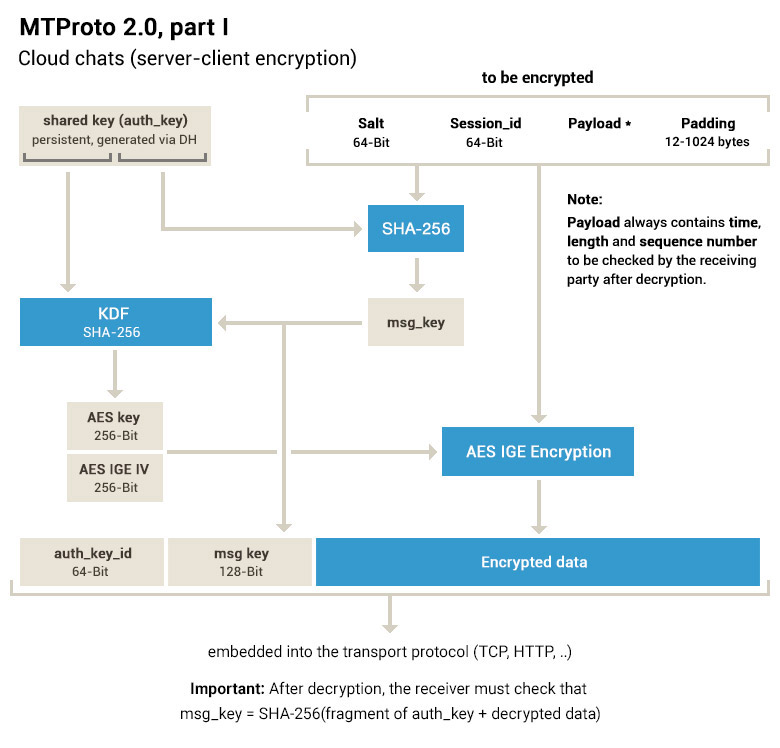
\includegraphics[scale=0.37]{../IMAGES/mproto1.jpeg}
        \caption{Схема MTProto v1 для хмарних чатів.}
        \label{mproto1}
\end{figure}

У даній роботі було наведено посилання \cite{telegramSecurityAnalysis} на роботи криптографів, що будували різні атаки на даний протокол. Цікаво, що у одній із них MTProto було визнано не є IND-CCA безпечним. Додамо, що даний протокол використовує RSA алгоритм для створення ключів та симетричний алгоритм AES.


Із приводу конфіденційності, то можна сказати, що Telegram:
\begin{itemize}
    \item може збирати пристойну кількість особистої інформації, яку він може зберігати до 12 місяців;
    \item відповідно до їх політики конфіденційності, вони, можуть такі метадані, як IP-адреса, пристрої та програми Telegram, якими ви користуєтеся, історія змін імені користувача тощо.
\end{itemize}


Окрім того, компанія має можливість читати будь-які ваші повідомлення Cloud Chat, щоб розслідувати спам та інші порушення їхніх умов обслуговування. Вони можуть ділитися деякими вашими особистими даними з іншими користувачами Telegram, з якими ви вирішите спілкуватися, і компаніями в групі Telegram. Якщо вимагатиметься рішення суду, вони можуть надати вашу IP-адресу та номер мобільного телефону відповідним органам. Це важливо мати на увазі під час використання Telegram.


Наступним розглянемо протокол \textbf{MTProto2} \cite{telegram_mtproto2}, що на даний час використовується для секретних та звичайних хмарних чатів. 

MTProto складається з кількох (під)протоколів, які обробляють початкову автентифікацію клієнтів зі створенням спільних ключів між клієнтами та сервером, створенням ключів сеансу між двома клієнтами для наскрізного шифрування в секретних чатах, повторним введенням секретних чатів і, звичайно, шифрування всіх повідомлень перед передачею через (можливо, незахищену) мережу.

Незважаючи на те, що MTProto 2.0 є повністю відкритим, а код клієнта відкритим, модель безпеки Telegram отримала широку критику. Перш за все, це через вибір нестандартного, спеціального протоколу та схеми шифрування викликав заперечення, тому що відсутність контролю може наражати систему на вразливість, потенційно підриваючи її безпеку. Крім того, усі повідомлення (навіть ті, що містяться в «секретних чатах») проходять через (хмару) пропрієтарні сервери із закритим кодом, де вони можуть зберігатися будь-який час. Ця архітектура зручна для користувачів, які можуть отримувати доступ до своїх повідомлень і синхронізувати їх із кількох пристроїв, а також надсилати й отримувати повідомлення навіть тоді, коли одноранговий пристрій відсутній, але з точки зору безпеки це означає, що сервер слід розглядати як ненадійну сторону.


Загалом MTProto v2 вважається безпечним і його більш детальний розбір можна знайти за посиланням \cite{miculan2021mtproto_v2}. Документ надає повністю автоматизоване підтвердження надійності автентифікації MTProto 2.0, звичайного та секретного чатів та механізмів повторного введення ключів, а також щодо властивостей безпеки: автентифікації, цілісність, конфіденційність й ідеальну пряму секретність. Це частково усуває занепокоєння щодо недостатньої перевірки, одночасно підтверджуючи формальну безпеку останньої версії протоколу.

\begin{figure}[ht]
        \centering
        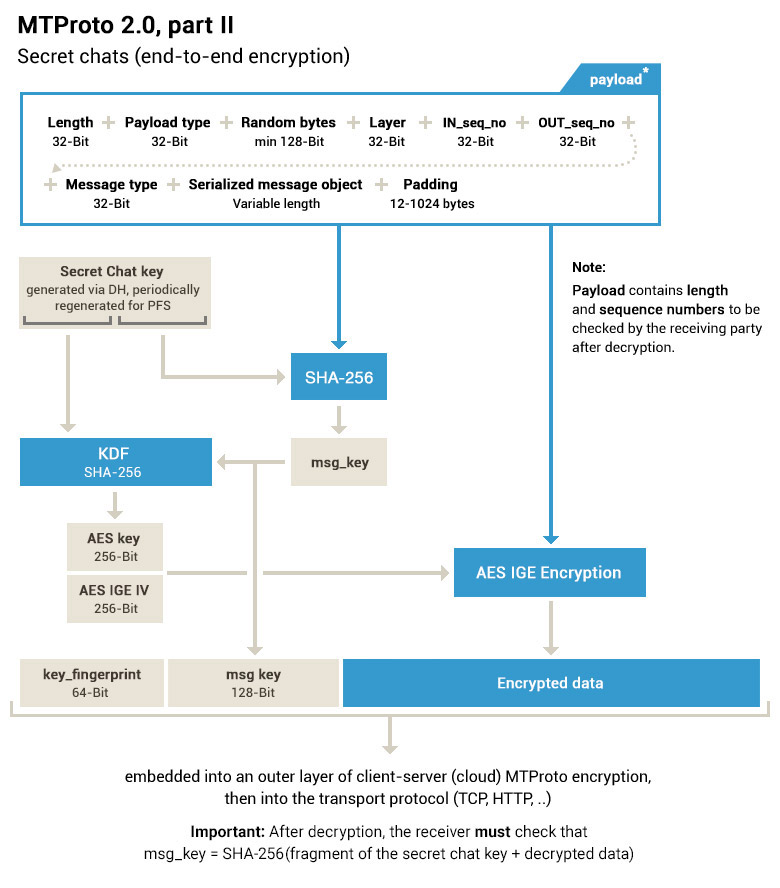
\includegraphics[scale=0.37]{../IMAGES/mproto2.jpeg}
        \caption{Схема MProto v2.}
        \label{mproto2}
\end{figure}

Тобто як узагальнити, то месенджер використовує дискретний логарифм для створення спільного ключа та загалом надійну схему протокола, що наведена у наступній схемі із урахуванням рівнів.

\begin{figure}[ht]
        \centering
        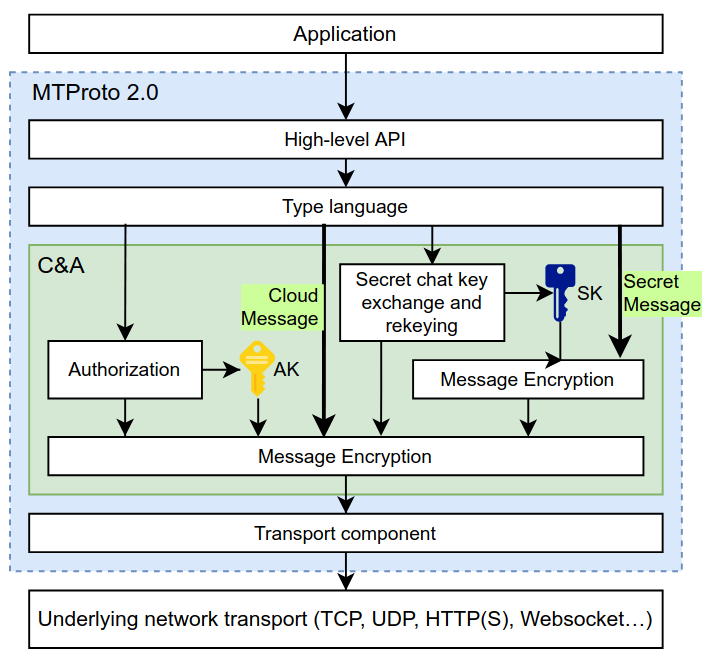
\includegraphics[scale=0.37]{../IMAGES/mtproto2_protocol.png}
        \caption{Рівні протоколу MProto v2.}
        \label{mproto2}
\end{figure}

Цю схему можна органічно поділити на 3 рівні, а саме:
\begin{itemize}
    \item \textbf{Прикладний рівень} -- визначає спосіб перетворення запитів і відповідей API
до двійкових повідомлень. Цей компонент відповідає рівням OSI 7 (application) і 6 (presentation).
    \item \textbf{Криптографічні та авторизаційні компоненти} - визначають, як користувачі автентифікуються на сервері, а повідомлення шифруються перед передачею через транспортний протокол. Ці компоненти відповідають рівням OSI 5 (session) і 4 (transport).
    \begin{itemize}
        \item Авторизація: цей модуль надає функціональні можливості для початкової авторизації клієнта та автентифікації сервера. Він викликається під час першого запуску програми для отримання ключа авторизації (AK), довгострокового <<головного>> секрету, який надається лише серверу. Щоб встановити ключ авторизації, цей модуль виконує криптографічний протокол (в основному обмін DH) із сервером.
        \item Обмін секретним ключем чату та зміна ключа: цей модуль надає функції для встановлення спільного секретного ключа сеансу (SK) між двома клієнтами. Він виконується один раз на початку секретного чату та після 100 обміну повідомленнями між двома сторонами (або протягом тижня) для встановлення нового ключа. В обох випадках цей модуль виконує обмін Діффі-Геллмана з одноранговим клієнтом (через сервер).
        \item Шифрування повідомлень: усі повідомлення між клієнтом і сервером шифруються за допомогою симетричного шифру з використанням ефемерного ключа, отриманого з AK. Повідомлення в секретних чатах також шифруються за допомогою ефемерного ключа, отриманого від SK. Схема шифрування однакова, але використовується двічі (з різними ключами) для повідомлень у секретних чатах.
    \end{itemize}
    \item \textbf{Транспортна компонента} -- визначає, як клієнт і сервер фактично обмінюються повідомленнями через існуючий транспортний протокол, такий як UDP, TCP, HTTP, HTTPS, WebSocket тощо. Варто зауважити, що також підтримуються незахищені протоколи без з’єднання.
\end{itemize}

\begin{figure}[ht]
        \centering
        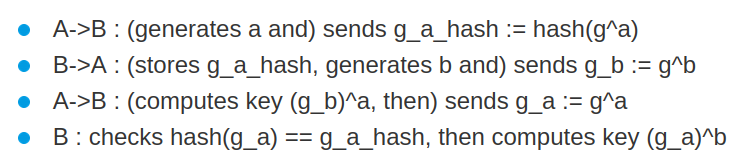
\includegraphics[scale=0.37]{../IMAGES/user_verification_mtproto2_calls.png}
        \caption{Схема автентифікації користувачів MProto v2 для дзвінків.}
        \label{mproto2_video}
\end{figure}

На останок додамо пару слів про аудіо та відео дзвінки \cite{telegram_mtproto2_video_calls}. У Telegram вони реалізовані за допомогою трохи модифікованої версії MTProto v2, що використовується у секретних чатах. У ній додано додаткову автентифікацію користувача за умови входження в онлайн, що є за замовчуванням, адже це є дзвінок. Обмін повідомленнями для автентифікації виглядає наступним чином \ref{mproto2_video}.

 % =================================== SECTION ===================================
\section{Viber}

\begin{wrapfigure}{l}{0.25\textwidth}
    
\includegraphics[width=0.9\linewidth]{../IMAGES/viber.png} 
    \label{fig:telegram}
\end{wrapfigure}

Viber, це крос-платформне програмне забезпечення для передачі голосу через IP (VoIP) і обміну миттєвими повідомленнями (IM), яке належить японській транснаціональній компанії Rakuten.

Голосові дзвінки, відеодзвінки, групові чати, стікери, соціальні канали, чати, що самознищуються, наскрізне шифрування, багато спаму та цільова реклама. Viber пропонує всі найкращі практики світу із програм обміну повідомленнями. Він схожий на суміш WhatsApp і Telegram із додаванням Snapchat. І це величезний додаток на понад мільярд користувачів у всьому світі. Під час пандемії Viber розширив функції групового відеочату, щоб дозволити більше користувачів, що призвело до появи цікавих речей, як-от вчителі в Угорщині використовували його, щоб підтримувати зв’язок зі своїми учнями. 

\subsection{Протоколи}
Viber досить добре захищає конфіденційність, адже у 2016 році за замовчуванням було прийнято наскрізне шифрування, окрім групових дзвінків. Тобто, якщо підсумувати, то наскрізне шифрування \cite{viber_end_to_end_encryption}:
\begin{itemize}
    \item використовується для
    \begin{enumerate}
        \item особистих повідомлень та дзвінків між двома абонентами;
        \item груп.
    \end{enumerate}
    
    \item не використовується для
    \begin{itemize}
        \item спільнот;
        \item каналів;
        \item чатів із ботами;
        \item групових дзвінків;
        \item платних дзвінків із Viber Out.
    \end{itemize}
\end{itemize}

E2E побудовано таким чином, що кожен пристрій користувача генерує 256-бітну Curve-25519 пару ключів, що зветься ID Key. Зокрема, за необхідності користувач генерує PreKey пару ключів для поширення їх на сервер та для іншого користувача.

\textbf{Сесії користувачів} між пристроями створюються тоді, коли пристрій перший раз реєструється. Тільки одна сесія потрібна для того, щоб синхронізувати будь-яку кількість повідомлень між двома акаунтами. 

У випадку, коли користувач A хоче встановити зв'язок із користувачем B, ініціатор отримує від сервера відповідні ID Key та PreKeys, що були попередньо згенеровані та відправлені на сервер іншим користувачем. Далі ініціатор генерує дві ключові пари по 256-біт Curve-25519 для рукостискання та для шифрування методом храповика відповідно. 


\begin{figure}[ht!]
        \centering
        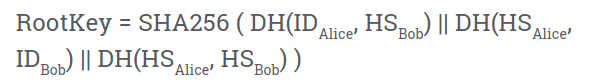
\includegraphics[scale=0.37]{../IMAGES/viber_1_root_key_deriving.png}
        \caption{Схема одержання RootKey.}
        \label{viber_1_root_key_deriving}
\end{figure}

\begin{figure}[ht!]
        \centering
        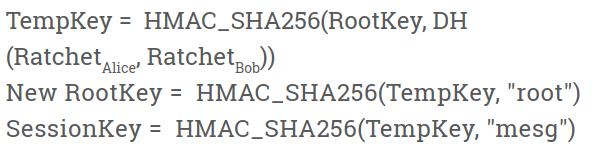
\includegraphics[scale=0.37]{../IMAGES/viber_2_session_key.png}
        \caption{Схема одержання ключа для сесії.}
        \label{viber_2_session_key}
\end{figure}

Різні рядки, передані до функцій HMAC запевняють нас, що навіть якщо ключ сеансу зламано, то кореневий ключ не може бути отриманий назад з нього.

Потім ініціатор надсилає користувачу Б повідомлення про початок сеансу, що містить його власний публічний ідентифікатор ID Key, ідентифікатор попереднього PreKey користувача Б, який використовувався для цього сеансу, а також його власні публічні ключі рукостискання та храповий ключ ініціатора. Коли користувач Б підключається до Інтернету та отримує це повідомлення він може реконструювати той самий кореневий і сеансовий ключі за допомогою тієї самої процедури DH.

Для \textbf{шифрування повідомлень}, як було згадано, використовується метод храповика. Для досягнення цього генерується ефемерний одноразовий 128-бітний симетричний ключ, який використовується для шифрування тіла повідомлення за допомогою алгоритму шифрування Salsa20. Потім цей ефемерний ключ повідомлення шифрується за допомогою сеансового ключа кожного одержувача. Пристрій-відправник надсилає уніфіковане повідомлення на сервер, що містить один зашифрований шифротекст і набір зашифрованих ефемерних ключів. Розгортання на стороні сервера розрізає це повідомлення та доставляє відповідні частини до кожного цільового пристрою. Два пристрої по черзі просувають сеансові ключі в процесі, який називається храповим механізмом. Кожного разу, коли напрямок розмови змінюється, пристрій, чия черга, випадковим чином генерує нову пару ключів Ratchet і знову виконує таку послідовність:

\begin{figure}[ht!]
        \centering
        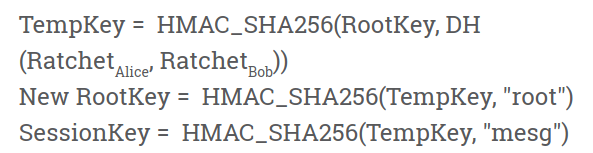
\includegraphics[scale=0.37]{../IMAGES/viber_3_msg_exchange.png}
        \caption{Схема одержання ключа для шифрування методом храповика.}
        \label{viber_3_msg_exchange}
\end{figure}

З $\text{Ratchet}_\text{this device}$ є приватною частиною щойно отриманої пари ключів. Разом із кожним повідомленням також надсилається загальнодоступна частина $\text{Ratchet}_{\text{this device}}$. Одержувач запускає DH зі своїм останнім приватним храповиком разом із публічним храповиком відправника.

Подвійний храповий механізм забезпечує дві речі: 
\begin{itemize}
    \item пряму та зворотну секретність, тож навіть якщо ключі скомпрометовані, минулі та майбутні повідомлення неможливо розшифрувати;
    \item алгоритм підтримує автентифікацію пристрою користувача, оскільки DH-ланцюжок кореневих ключів починається з ID Keys обох пристроїв. Якщо ID Keys однорангового вузла є надійним у будь-який момент, то всьому ланцюжку можна довіряти.
\end{itemize}

\subsection{Репутація}

Загалом Viber має в Україні одну з найбільших спільнот користувачів, а саме 9 мільйонів. Не дивлячись на велику підтримку України, можна сказати, що це є тим месенджером, якому можна довіряти. Із іншого боку Сили Оборони України не довіряють йому і користуються альтернативними месенджерами. Зокрема, нещодавно була здійснена атака із викраденням 740 гігабайтів даних із месенджера \ref{hackread2025viber}. У документації бракує детальнішого опису алгоритмів, щоб зрозуміти доцільність використання даного месенджера.


 % =================================== SECTION ===================================
\section{Signal}

\begin{wrapfigure}{l}{0.25\textwidth}
    
\includegraphics[width=0.9\linewidth]{../IMAGES/signal.png} 
    \label{fig:signal}
\end{wrapfigure}

Signal - це відкрите програмне забезпечення із обміну зашифрованими миттєвими повідомленнями, голосовими дзвінками та відеодзвінками. Функція обміну миттєвими повідомленнями включає надсилання тексту, голосових нотаток, зображень, відео та інших файлів. Спілкування між користувачами може бути індивідуальним або передбачати груповий обмін повідомленнями. 

Додамо, що Відповідно до Signal, він «ні в якому разі не продає, не здає в оренду та не монетизує ваші особисті дані чи контент». Signal реалізує принципи мінімізації даних - лише номер телефону використовується як джерело даних - і захисту даних за замовчуванням і за проектом.

\subsection{Протоколи}

Створення безпечного протоколу обміну повідомленнями не могло обійтися без використання складних схем шифрування та обміну даними. Його називають як стеком протоколів Signal і, як мінімум, використовує WhatsApp для свого функціонування. Обговоримо технічні деталі, що були використані для його реалізації.

\begin{itemize}
    \item XEdDSA та VXEdDSA

        XEdDSA та VXEdDSA — це схеми криптографічного підпису, розроблені для уніфікації форматів ключів для операцій еліптичної кривої Діффі-Геллмана (ECDH) і алгоритму цифрового підпису Едвардса (EdDSA). У деяких ситуаціях це дозволяє використовувати ту саму пару ключів для обох алгоритмів.

        \textit{XEdDSA} полегшує використання однієї пари ключів як для операцій ECDH, так і для EdDSA, спрощуючи керування ключами та зменшуючи потребу в кількох парах ключів. Також дозволяє створювати та перевіряти підписи, сумісні з EdDSA, використовуючи ключові формати, спочатку визначені для функцій Діффі-Геллмана на еліптичній кривій X25519 і X448.

        \textit{VXEdDSA} розширює XEdDSA шляхом включення керування версіями, дозволяючи схемі функціонувати як перевірена випадкова функція (VRF). На додаток до перевірки підпису, за успішного завершення, VXEdDSA повертає результат VRF, який гарантовано буде унікальним для повідомлення та відкритого ключа. Вихідні дані VRF для даного повідомлення та відкритого ключа неможливо відрізнити від випадкових для тих, хто не бачив підпис VXEdDSA для цього повідомлення та ключа.

        Додамо, що детальніше нюанси реалізації можна побачити за цим посиланням \cite{perrin2016xeddsa}.
        
    \item X3DH 

        X3DH (або Extended Triple Diffie-Hellman) - це схема узгодження ключів, що встановлює спільний секретний ключ між двома сторонами, які взаємно автентифікують одна одну на основі відкритих ключів. X3DH забезпечує пряму секретність і криптографічну заборону.

        X3DH розроблено для асинхронних налаштувань, коли один користувач (<<Боб>>) перебуває в автономному режимі, але опублікував певну інформацію на сервері. Інший користувач (<<Аліса>>) хоче використати цю інформацію для надсилання зашифрованих даних Бобу, а також створити спільний секретний ключ для майбутнього спілкування.
        
        \begin{figure}[ht!]
            \centering
            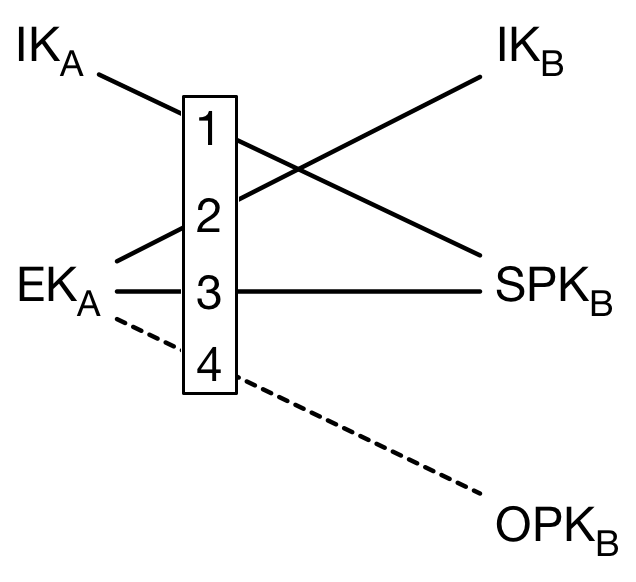
\includegraphics[scale=0.8]{../IMAGES/signal_X3DH.png}
            \caption{Схема обміну ключами для X3DH.}
            \label{signal_X3DH}
        \end{figure}

        Уточнимо, що IK - індентифікаційний ключ, SPK - попередньо підписаний попередній ключ, EK~-~ефемерний ключ, OPK - одноразовий передключ.

        Додамо, що детальніше нюанси реалізації можна побачити за цим посиланням \cite{marlinspike2016x3dh}.
        
    \item PQXDH 

        PQXDH (або Post-Quantum Extended Diffie-Hellman) - протокол узгодження ключів, що встановлює спільний секретний ключ між двома сторонами, які взаємно автентифікують одна одну на основі відкритих ключів. PQXDH забезпечує постквантову пряму секретність і певну форму криптографічного заперечення, але все ще покладається на складність проблеми дискретного логарифмування для взаємної автентифікації.

        PQXDH розроблено для асинхронних налаштувань, коли один користувач (<<Боб>>) перебуває в автономному режимі, але опублікував певну інформацію на сервері. Інший користувач (<<Аліса>>) хоче використати цю інформацію для надсилання зашифрованих даних Бобу, а також створити спільний секретний ключ для майбутнього спілкування.

        Додамо, що детальніше нюанси реалізації можна побачити за цим посиланням \cite{kret2023pqxdh}
    
    \item Double Ratchet 

        Double Ratchet - криптографічний протокол, який використовується двома сторонами для обміну зашифрованими повідомленнями на основі спільного секретного ключа. Як правило, сторони використовують певний протокол узгодження ключів (наприклад, X3DH), щоб узгодити спільний секретний ключ. Після цього сторони використовуватимуть Double Ratchet для надсилання та отримання зашифрованих повідомлень.

        Сторони отримують нові ключі для кожного повідомлення Double Ratchet, щоб попередні ключі не можна було обчислити з пізніших. Сторони також надсилають загальнодоступні цінності Діффі-Геллмана, додані до своїх повідомлень. Результати обчислень Діффі-Геллмана змішуються з похідними ключами, щоб пізніші ключі не можна було обчислити з попередніх. Ці властивості надають певний захист попереднім або пізнішим зашифрованим повідомленням у разі зламу ключів сторони.

        \begin{figure}[ht!]
            \centering
            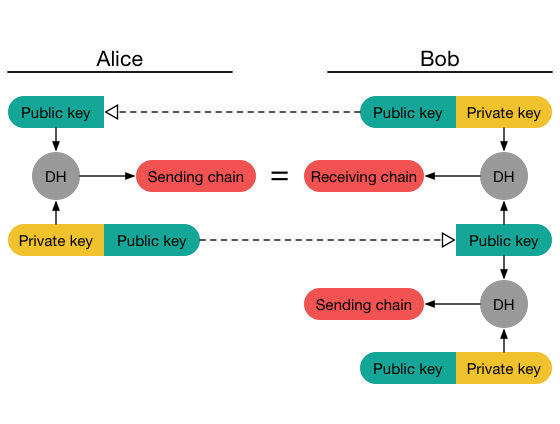
\includegraphics[scale=0.5]{../IMAGES/signal_double_ratchet1.png}
            \caption{Схема створення нових ключів для шифрування у Double Ratchet.}
            \label{signal_double_ratchet1}
        \end{figure}
    
        Додамо, що детальніше нюанси реалізації можна побачити за цим посиланням \cite{perrin2016doubleratchet}
    
    \item Sesame 

        Алогоритм Sesame - це протокол для керування сеансами шифрування повідомлень в асинхронних налаштуваннях із кількома пристроями.

        Sesame був розроблений для керування сесіями Double Ratchet, створеними за допомогою угоди ключа X3DH. Він координує створення, видалення та використання сеансів шифрування на кількох пристроях, забезпечуючи безпечний і синхронізований зв’язок.


        Sesame:
        \begin{itemize}
            \item підтримує активні сеанси шифрування між пристроями, сприяючи безперебійному обміну повідомленнями, навіть якщо деякі пристрої перебувають у режимі офлайн;
            \item ефективно обробляє сценарії, коли користувачі працюють з кількома пристроями, гарантуючи, що повідомлення належним чином зашифровані та доставлені на кожен пристрій;
            \item гарантує, що кожен пристрій підтримує «активний» сеанс для кожного іншого пристрою, з яким він спілкується, гарантуючи, що повідомлення шифруються за допомогою правильних ключів сеансу;
            \item гарантує, що коли повідомлення отримано під час неактивного сеансу, цей сеанс стає активним, дозволяючи пристроям синхронізуватися та узгодити відповідний сеанс для використання;
            \item керує життєвим циклом сеансів, створюючи нові під час додавання пристроїв і видаляючи їх, коли пристрої видаляються, зберігаючи цілісність комунікаційної мережі.
        \end{itemize}
        
        
        Однак Sesame — це загальний алгоритм, який працює з будь-яким алгоритмом шифрування повідомлень на основі сеансу, який відповідає певним умовам.
        
        Додамо, що детальніше нюанси реалізації можна побачити за цим посиланням \cite{marlinspike2017sesame}
\end{itemize}

Цікаво, але для Signal протоколів теж існують роботи із аналізу безпеки, а саме:
\begin{itemize}
    \item Формальний аналіз безпеки Signal протоколу обміну\cite{cohn-gordon2016formal}
    \item та інші \dots
\end{itemize}


\subsection{Підсумки}

Загалом це є одним із найкращих на даний момент месенджерів, що не збирає жодних даних і є орієнтований на анонімне використання. Звичайно, цей додаток не має жодних інтеграцій із бізнесами, що не дає поширювати комерційну інформацію серед них. 

 % =================================== SECTION ===================================
\section{WhatsApp}

\begin{wrapfigure}{r}{0.25\textwidth}
    
\includegraphics[width=0.9\linewidth]{../IMAGES/whatsapp.png} 
    \label{fig:whatsapp}
\end{wrapfigure}

WhatsApp Messenger — це служба обміну миттєвими повідомленнями і передачі голосу через IP, що належить технологічному конгломерату Meta. Це дозволяє користувачам надсилати текстові, голосові та відеоповідомлення, здійснювати голосові та відеодзвінки, а також ділитися зображеннями, документами, місцезнаходженням користувачів та іншим вмістом. Послуга вимагає номер стільникового мобільного телефону для реєстрації.[19] У січні 2018 року WhatsApp випустив окрему бізнес-програму під назвою WhatsApp Business, яка може спілкуватися зі стандартним клієнтом WhatsApp.

WhatsApp був заснований Яном Кумом і Брайаном Ектоном, які раніше 20 років разом працювали в Yahoo. WhatsApp приєднався до Facebook у 2014 році, але продовжує працювати як окрема програма з фокусом на створенні служби обміну повідомленнями, яка працює швидко та надійно в будь-якій точці світу.

\subsection{Протоколи}

WhatsApp використовує Signal протоколи, що були проаналізовані та протестовані усіма можливими дослідниками. Вони вважаються на даний час одними із найкращих. Додам, що даний месенджер використовує реалізацію протоколів, але реалізація додатку залишається за компанією. Відповдіно до запису у блозі Signal, WhatsApp перейшов на наскрізне шифрування аж у 2016 році, що каже про обізнаність розробників \cite{moxie02016whatsapp}.


\begin{figure}[ht!]
        \centering
        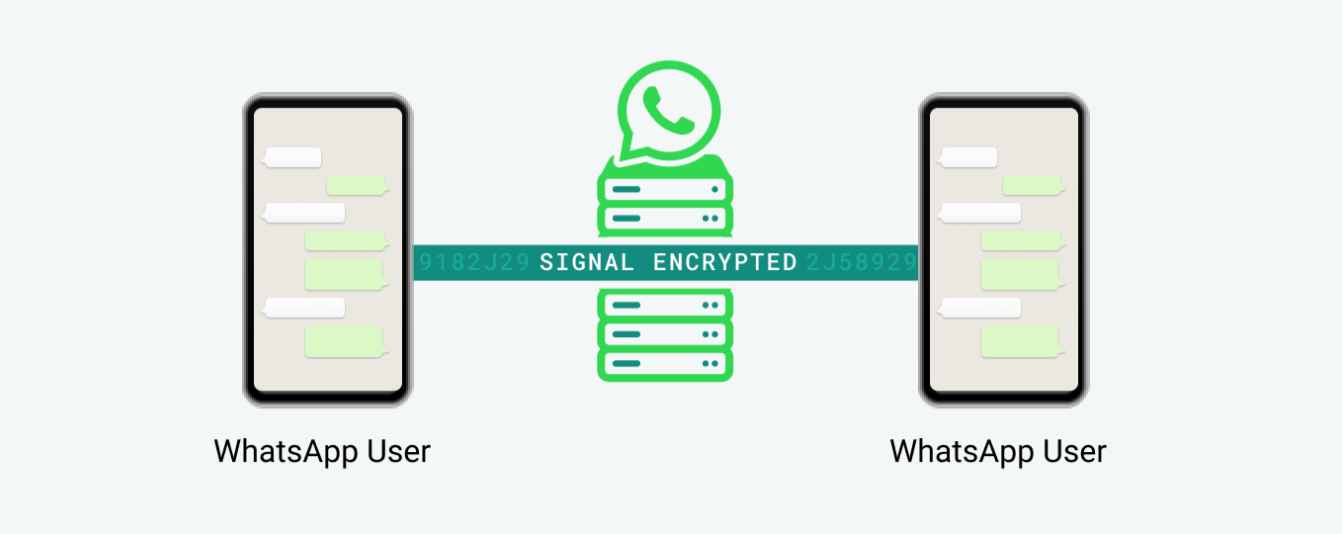
\includegraphics[scale=0.37]{../IMAGES/whatsapp_ordinary_comunication.png}
        \caption{Схема комунікації користувачів як через звичайну мережу так і через мережу бізнесів.}
        \label{whatsapp_ordinary_communication}
\end{figure}

Неможливо не сказати про схему реалізації спілкування користувачів між користувачами та бізнесами. Перший рисунок показує схему спілкування звичайних користувачів із собі ж подібними на загальній мережі. Тобто всі повідомлення певним чином маршрутизуються та оброблюються розгорнутим сервером WhatsApp. У WhatsApp Business можна користуватися чатом, що має більше можливостей, ніж звичайний, для просування власних потреб у ньому \ref{whatsapp_ordinary_communication}. 

\begin{figure}[ht!]
        \centering
        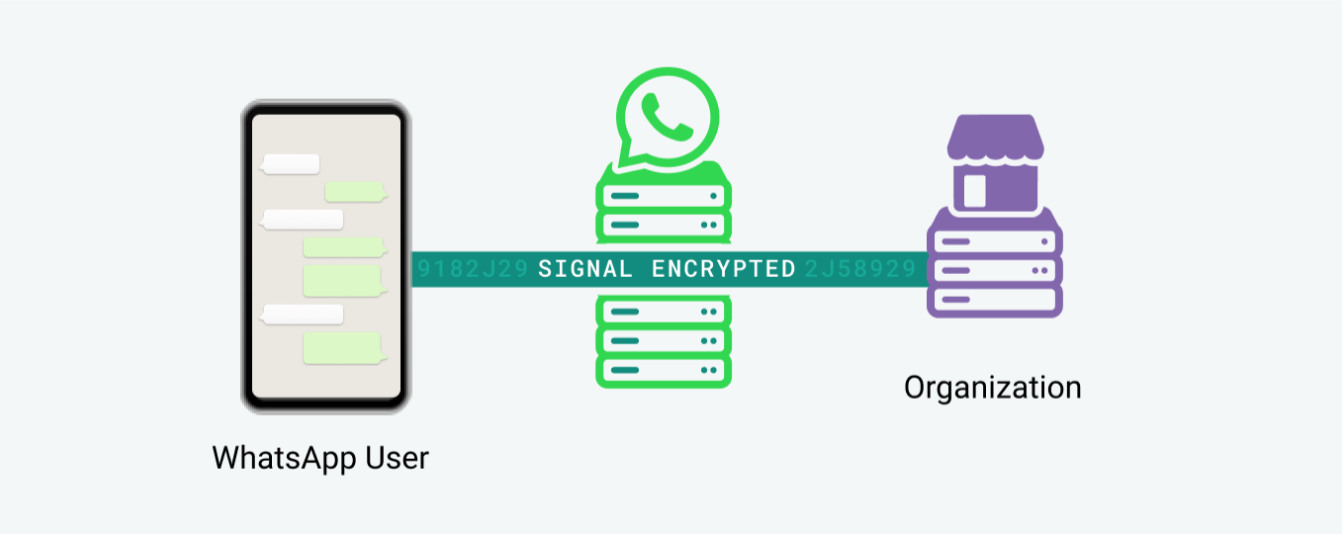
\includegraphics[scale=0.37]{../IMAGES/whatsapp_organization_communication.png}
        \caption{Схема отримання даних для біснесу на їхні сервери.}
        \label{whatsapp_organization_communication}
\end{figure}

Деякі організації можуть використовувати локальний WhatsApp Business API додаток \ref{whatsapp_organization_communication}, який можна розгорнути як кінцеву точку WhatsApp на сервері. API дозволяє цим організаціям програмно надсилати й отримувати повідомлення.

WhatsApp вважає зв’язок із локальними користувачами WhatsApp Business API, які керують кінцевою точкою API на серверах, наскрізно зашифрованим, оскільки немає стороннього доступу до вмісту між кінцевими точками.

Підсумовуючи, наведемо список із знайдених досліджень щодо стійкості імплементованого месенджера:
\begin{itemize}
    \item Документ, що дає зрозмути які алгоритми шифрування використовуються \cite{whatsapp2024encryption}.
    \item Побудова атак на протокол реєстрацiї супутнього пристрою в WhatsApp \cite{nemkovich2023whatsapp}.
    \item Порівняння аналізу безпеки між Signal, WhatsApp і Telegram \cite{bogos2023security}.
    \item Аналіз документів безпеки WhatsApp \cite{li2016whatsapp}.
    \item Інший аналіз безпеки від International Journal of Science and Research \cite{alhameed2018whatsapp}.
    \item Аналіз безпеки протоколу наскрізного шифрування резервного копіювання \cite{davies2023security}.
\end{itemize}


\subsection{Підсумки}

Як узагальнемо, то WhatsApp є надійним месенджером, що він надає надійні гарантії безпеки як і для бізнесу так і для особистого спілкування. Єдине на що треба зважати, це збір даних який все таки трохи відбувається через Meta для покращення власних сервісів.


 % =================================== SECTION ===================================
\section{Різниця Signal та WhatsApp}

Не дивлячись на те, що WhatsApp також використовує Signal протокол для обміну повідомленнями, проте вони мають у собі певні різниці:

\begin{itemize}
    \item \textbf{Право володіння}
        \begin{itemize}
            \item \textbf{\textit{Signal}}
                
                Належить некомерційній організації Signal Foundation, яка діє як неприбуткова організація та фінансується за рахунок пожертвувань та грантів. Немає жодної реклами, відстеження чи монетизації даних користувачів.

            \item \textbf{\textit{WhatsApp}}
                
                Належить Meta (або раніше Facebook). Бізнес-модель передбачає інтеграцію з ширшою екосистемою Meta, включаючи потенційний обмін даними (хоча чати WhatsApp залишаються зашифрованими).
        \end{itemize}
    
    \item \textbf{Збирання даних}
        \begin{itemize}
            \item \textbf{\textit{Signal}}
                
                Збирає мінімум метаданих (до прикладу, номер телефону та час створення облікового запису). Не збирає та не зберігає історію чату чи дані користувача.
            \item \textbf{\textit{WhatsApp}}
                
                Збирає більше метаданих: номери телефонів, контакти, інформацію про пристрій і статистику використання. Ділиться деякими даними з Meta для аналітики та бізнес-інтеграції.
        \end{itemize}
        
    \item \textbf{Безпека}
        \begin{itemize}
            \item \textbf{\textit{Signal}}
                
                Використовує свій відкритий протокол сигналу для наскрізного шифрування (E2EE). Повідомлення, дзвінки, групові чати та мультимедійні дані є зашифрованими. У месенджері немає резервних копій або хмарної синхронізації повідомлень, якщо вони явно не були експортовані користувачем.
            \item \textbf{\textit{WhatsApp}}
                
                Також використовує протокол сигналу для E2EE. Повідомлення, дзвінки та групові чати шифруються за замовчуванням. Резервні копії, що зберігаються в хмарних службах, не шифруються, якщо користувач не ввімкне резервне копіювання з наскрізним шифруванням.
        \end{itemize}
        
    \item \textbf{Особливості та фокус}
        \begin{itemize}
            \item \textbf{\textit{Signal}}
               
                Орієнтований на конфіденційність і простоту. Пропонує такі функції, як зникнення повідомлень, анонімний обмін повідомленнями (без спільного доступу до контактів) і безпечні PIN-коди. Немає широких бізнес або соціальних функцій.
            \item \textbf{\textit{WhatsApp}}
                
                Призначений для більш широкого використання, включаючи соціальне та ділове спілкування. Пропонує такі функції, як WhatsApp Business \cite{whatsapp_business}, канали, оновлення статусу та зашифровані резервні копії. Поєднує безпеку зі зручністю для користувача та соціальною залученістю.
        \end{itemize}
        
    \item \textbf{Відкритість вихідних кодів}
        \begin{itemize}
            \item \textbf{\textit{Signal}}
                
                Повністю відкритий вихідний код, тобто його код є загальнодоступним для вивчення та модифікації.
            \item \textbf{\textit{WhatsApp}}
                
                Частково з відкритим вихідним кодом, але більшість його коду та внутрішніх операцій залишаються запатентованими.
        \end{itemize}
        
    \item \textbf{База користувачів}
        \begin{itemize}
            \item \textbf{\textit{Signal}}
                
                Приваблює користувачів, які надають пріоритет конфіденційності, безпеці та некомерційній етиці. Менша база користувачів порівняно з WhatsApp.
            \item \textbf{\textit{WhatsApp}}
                
                Один із найпоширеніших додатків для обміну повідомленнями в усьому світі з мільярдами користувачів. Більш широке впровадження та інтеграція з бізнесом.
        \end{itemize}
        
    \item \textbf{Signal протокол}
        \begin{itemize}
            \item \textbf{\textit{Signal}}
                
                Signal переважно використовує реалізацію протоколу Signal (libsignal) \cite{libsignal_rust}, що імплементована на Rust у його сучасних версіях. Перевага віддається Rust через його продуктивність, гарантії безпеки та строгу систему типів.
            \item \textbf{\textit{WhatsApp}}
                
                Відомо, що WhatsApp використовує реалізацію Java протоколу сигналів (libsignal-protocol-java) \cite{libsignal_protocol_java} у своїх Android і серверних системах. Бібліотека Java добре інтегрується з існуючою інфраструктурою WhatsApp, яка значною мірою покладається на Java для серверних служб і розробки Android.
        \end{itemize}
        
\end{itemize}


 % =================================== CHAPTER ===================================
\chapter{Конфіденційність за проектуванням}

На останок можна згадати роботу дослідників, що сформували документ у якому містяться пункти про те, як треба робити безпечні додатки. Розберемо коротко 7 основоположних принципів конфіденційності за проектуванням \cite{cavoukian_privacy_by_design}:

\begin{itemize}
    % \setlength{\parindent}{0pt} % Disable paragraph indentation

    \item \textbf{Проактивний, а не реактивний; Профілактичний, а не лікувальний}
    
    Це означає, що програмне забезпечення має залишатися підтримуваним, а розробники - зобов’язаними, як з огляду на законодавство, так і з огляду на суспільну культуру, дотримуватися найкращих практик захисту інформації. Важливо діяти на випередження, а не обмежуватися реактивними заходами.
    
    \item \textbf{Конфіденційність за замовчуванням}

    Означає використання мінімізації зібраних особистих даних, детальне аргументування для чого вони потрібні, відкриття певних даних лише у законних цілях за проханням держави і безпечно утилізовані.
    
    \item \textbf{Конфіденційність влаштована у дизайн проекту}

    Конфіденційність повинна бути влаштована у дизайн цілісної системи, щоб при помилці, взламі мінімізувати витік даних. Зокрема повинно бути пом'якшено ризики, що зв'язані із можливими векторами атак на конфіденційність додатку.
    
    \item \textbf{Повна функціональність}

    Конфіденціність за проектуванням за своєю природою забезпечує подвійні можливості, дозволяючи повну функціональність, а саме реальні практичні результати та вигідні результати для кількох сторін. Мається на увазі, що користувачам повнно бути надано повний функціонал додатку без урізання можливостей із захисту даних.
    
    \item \textbf{Наскрізне шифрування}

    Конфіденційність має постійно захищати в усьому домені та протягом життєвого циклу даних. Організації повинні нести відповідальність за безпеку особистої інформації відповідно до ступеня чутливості протягом усього життєвого циклу відповідно до стандартів. І звичайно треба дотримуватися правильності видалення/зберігання/розповсюдження даних.
    
    \item \textbf{Видимість та порозорість}

    Означає використання підзвітності щодо того як дані є зшифровані чи куди були передані для зберігання, відкритості задля легкої перевірки, відповідності дій відповідно до задокументованих процедур доступу до інформації.
    
    \item \textbf{Повага до конфіденційності користувачів}

    Означає урахування інтересів і потреб окремих користувачів, які найбільше зацікавлені в управлінні своїми особистими даними. Надання можливості суб’єктам даних відігравати активну роль в управлінні своїми власними даними.
    
\end{itemize}